\documentclass[tikz,border=5pt]{standalone}
\usepackage{amssymb,amsmath}
\newcommand{\C}{\mathbb{C}}
\newcommand{\CP}{\mathbb{CP}}
\newcommand{\Res}{\operatorname{Res}}
\begin{document}
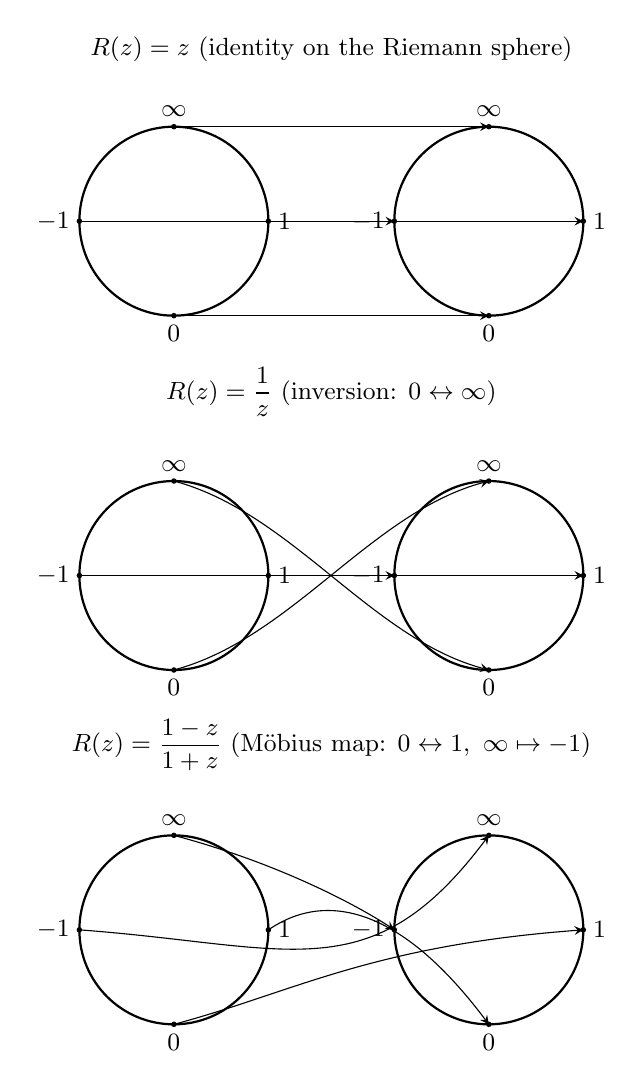
\begin{tikzpicture}[font=\small,>=stealth]
	
	\tikzset{
		sphere/.style={thick},
		spoint/.style={circle,fill,inner sep=1.2pt},
	}
	
	% Macro: draw a sphere with 4 marked points (∞, 0, 1, -1)
	% Arguments: center x, center y, name prefix
	\newcommand{\SphereFour}[3]{%
		% Circle (Riemann sphere in 2D)
		\draw[sphere] (#1,#2) circle (1.2);
		% Coordinates for the 4 special points
		\coordinate (#3N) at (#1,#2+1.2); % north: infinity
		\coordinate (#3S) at (#1,#2-1.2); % south: 0
		\coordinate (#3E) at (#1+1.2,#2); % east: 1
		\coordinate (#3W) at (#1-1.2,#2); % west: -1
		% Draw points
		\fill[spoint] (#3N) circle (1pt);
		\fill[spoint] (#3S) circle (1pt);
		\fill[spoint] (#3E) circle (1pt);
		\fill[spoint] (#3W) circle (1pt);
		% Labels
		\node[above] at (#3N) {$\infty$};
		\node[below] at (#3S) {$0$};
		\node[right] at (#3E) {$1$};
		\node[left]  at (#3W) {$-1$};
	}
	
	%========================================
	% Panel 1: R(z) = z (identity)
	%========================================
	\begin{scope}[shift={(0,4.5)}]
		
		\node[above] at (0,1.9) {$R(z)=z$ (identity on the Riemann sphere)};
		
		% Left sphere (domain) and right sphere (codomain)
		\SphereFour{-2}{0}{A}
		\SphereFour{ 2}{0}{B}
		
		% Arrows: each special point maps to itself
		\draw[->] (AN) -- (BN);
		\draw[->] (AS) -- (BS);
		\draw[->] (AE) -- (BE);
		\draw[->] (AW) -- (BW);
		
	\end{scope}
	
	%========================================
	% Panel 2: R(z) = 1/z
	%========================================
	\begin{scope}[shift={(0,0)}]
		
		\node[above] at (0,1.9)
		{$R(z)=\dfrac{1}{z}$ (inversion: $0\leftrightarrow\infty$)};
		
		% Domain and codomain spheres
		\SphereFour{-2}{0}{C}
		\SphereFour{ 2}{0}{D}
		
		% Mapping of special points:
		% R(0)   = ∞
		% R(∞)   = 0
		% R(1)   = 1
		% R(-1)  = -1
		
		% 0 -> ∞
		\draw[->] (CS) .. controls (-0.5,-0.8) and (0.5,0.8) .. (DN);
		% ∞ -> 0
		\draw[->] (CN) .. controls (-0.5,0.8) and (0.5,-0.8) .. (DS);
		% 1 -> 1
		\draw[->] (CE) -- (DE);
		% -1 -> -1
		\draw[->] (CW) -- (DW);
		
	\end{scope}
	
	%========================================
	% Panel 3: R(z) = (1 - z)/(1 + z)
	%========================================
	\begin{scope}[shift={(0,-4.5)}]
		
		\node[above] at (0,1.9)
		{$R(z)=\dfrac{1-z}{1+z}$ (Möbius map: $0\leftrightarrow 1,\ \infty\mapsto -1$)};
		
		% Domain and codomain spheres
		\SphereFour{-2}{0}{E}
		\SphereFour{ 2}{0}{F}
		
		% Images of special points:
		% R(0)    =  1
		% R(1)    =  0
		% R(\infty) = -1          (from leading terms)
		% R(-1)   =  ∞            (denominator 0)
		
		% 0 -> 1
		\draw[->] (ES) .. controls (-0.5,-0.8) and (0.5,-0.2) .. (FE);
		% 1 -> 0
		\draw[->] (EE) .. controls (-0.5,0.2) and (0.5,0.8) .. (FS);
		% ∞ -> -1
		\draw[->] (EN) .. controls (-0.5,0.8) and (0.5,0.2) .. (FW);
		% -1 -> ∞
		\draw[->] (EW) .. controls (-0.5,-0.2) and (0.5,-0.8) .. (FN);
		
	\end{scope}
	
\end{tikzpicture}
\end{document}